%%%%%%%%%%%%%%%%%%%%%%%%%%%%%%%%%%%%%%%%%
% University Assignment Title Page 
% LaTeX Template
% Version 1.0 (27/12/12)
%
% This template has been downloaded from:
% http://www.LaTeXTemplates.com
%
% Original author:
% WikiBooks (http://en.wikibooks.org/wiki/LaTeX/Title_Creation)
%
% License:
% CC BY-NC-SA 3.0 (http://creativecommons.org/licenses/by-nc-sa/3.0/)
% 
% Instructions for using this template:
% This title page is capable of being compiled as is. This is not useful for 
% including it in another document. To do this, you have two options: 
%
% 1) Copy/paste everything between \begin{document} and \end{document} 
% starting at \begin{titlepage} and paste this into another LaTeX file where you 
% want your title page.
% OR
% 2) Remove everything outside the \begin{titlepage} and \end{titlepage} and 
% move this file to the same directory as the LaTeX file you wish to add it to. 
% Then add \input{./title_page_1.tex} to your LaTeX file where you want your
% title page.
%
%%%%%%%%%%%%%%%%%%%%%%%%%%%%%%%%%%%%%%%%%
%\title{Title page with logo}
%----------------------------------------------------------------------------------------
%	PACKAGES AND OTHER DOCUMENT CONFIGURATIONS
%----------------------------------------------------------------------------------------

\documentclass[23pt]{article}
\usepackage[margin=1in, paperwidth=21cm, paperheight=29.7cm]{geometry}
\usepackage[pdftex]{color,graphicx}
\usepackage[english]{babel}
\usepackage[utf8x]{inputenc}
\usepackage{amsmath}
\usepackage[colorinlistoftodos]{todonotes}
\usepackage{cite}
\usepackage{listings}
\usepackage[nodayofweek]{datetime}
\usepackage{setspace}
\usepackage{fancyhdr}
\newcommand{\HRule}{\rule{\linewidth}{0.5mm}}
\begin{document}
\nocite{*}
\pagenumbering{roman}
\title{\begin{center}
\bf SEMINAR REPORT\\
\vspace{0.5cm} On\\
\HRule \\[0.4cm]
{ \huge \bfseries Google Cloud Messaging}\\[0.4cm] % Title of your document
\HRule \\[0.4 cm]
\vspace{0.5cm} \begin{Large} Submitted by:\\ 
\vspace{.35cm}Kevin Joseph (13400032)
\end{Large}
\end{center}}
\vspace{.5cm}
\date{}

\maketitle
\begin{center}
 {\it\large for the award of the degree}
\end{center}
\begin{center}
 {\it\large of}
\end{center}
\begin{center}
 {\bf\Large Bachelor of Technology}
\end{center}

\begin{center}

\includegraphics[scale=.8]{images/logo.jpg}
\end{center}
\vspace{.28cm}

\begin{center}
{\bf\large DEPARTMENT OF COMPUTER SCIENCE AND ENGINEERING}

\vspace{.35cm}
{\bf\large COLLEGE OF ENGINEERING\ , TRIVANDRUM}
\begin{center}{\large \formatdate{19}{7}{2016}}\\[1cm]\end{center}
\end{center}

\newpage

\begin{center}
{\bf{\LARGE CERTIFICATE}}
\end{center}
\vspace{.1cm}
\begin{center}

\includegraphics[scale=.45]{images/logo.jpg}
\end{center}
\begin{center}
\textbf{\Large College of Engineering,
Trivandrum}
\end{center}

\vspace{.6cm}
\begin{Large}
\begin{spacing}{1.5}
\hspace{1.5cm} This  is  to certify that the seminar entitled {\bf Google Cloud Messaging} done by {\bf  Kevin Joseph (13400032)} of the {\bf Department of Computer Science and Engineering, College of Engineering, Trivandrum} in partial fulfillment of the requirements for the award of the degree of Bachelor of Technology in Computer Science and Engineering under Kerala University is a Bonafide record of work carried out by him.
\vspace{2cm}
\end{spacing}

\bf\Large \hspace{.3cm}\hspace{1.7cm} \hspace{3cm} \\
\bf\Large \hspace{1cm}Seminar Co-ordinator    \hspace{4cm} Head of Department

\vspace{2cm}
\begin{spacing}{1.4}
\noindent Place : Trivandrum

\noindent Date \ : \formatdate{19}{7}{2016}
\end{spacing}
\end{Large}

\newpage
\pagenumbering{roman}
\begin{center}
\bf{{\LARGE ACKNOWLEDGEMENT}}
\end{center}
\begin{Large}
\begin{spacing}{1.1}
\vspace{1cm}
\hspace{2cm}
It is with great enthusiasm and spirit I am bringing out this seminar report. First and foremost I wish to express my wholehearted indebtedness to God Almighty for his gracious  blessings showered upon me.

\hspace{2cm} 
I am extremely grateful for the constant guidance rendered to me by Dr. Abdul Nizar, Head Of the Department of Computer Science, College of Engineering, Trivandrum , our seminar coordinators Mr. Vipin Vasu A. V. and Mr. Sreelal S. . I would also like to express my sincere gratitude to each member of Dept. of Computer Science, GEC, Palakkad for their kind co-operation and encouragement that helped me in completing the seminar. Last but not the least, I would like to thank my friends and parents who have given constant encouragement throughout the course of this project.
\end{spacing}
\end{Large}
\newpage
\begin{center}{\bf{\LARGE ABSTRACT}}
\end{center}
\begin{Large}
\begin{spacing}{1.1}
Android traditionally kept data synchronization between android-device and server-side using a method of pulling. Each 
		Android device has to poll the server for updated data, which leads to unneccessary network traffic
		and wastage of device battery. In order to overcome this weakness, a data pushing service, GCM was introduced.
		Push describes a style of communication where the request for a given transaction is initiated by the publisher
		or central server. Push messaging is a multi-channel mobile cloud communication platform that unifies push
		notifications, SMS and instant messaging.\\ GSM service allows sending data from the app engine or 
		any other backend to android powered devices. GSM is a lightweight push notification based service notifying
		android applications about new data to be fetched from the server or sending messages containing 4KB
		of payload data. GCM manages all aspects of message queuing and delivery of message to target android
		application running on a target device. Applications on the target device need not be running to receive
		messages. This service will wake up the application as long as the application is set up with the proper broadcast 
		receiver and permissions. The application might post a
		notification, display a custom user interface,
		or silently sync data.
\end{spacing}
\end{Large}

\newpage
\tableofcontents
\listoffigures
\newpage
\renewcommand{\abstractname}{\Large Abstract}
	
\newpage
\pagenumbering{arabic}
\section{Introduction to Cloud}
Cloud computing is a kind of Internet-based computing that provides shared processing resources and data to computers and other devices on demand. It is a model for enabling ubiquitous, on-demand access to a shared pool of configurable computing resources (e.g. networks, servers, storage, applications and services)\cite{dcc}\cite{4} which can be rapidly provisioned and released with minimal management effort. Cloud computing and storage solutions provide users and enterprises with various capabilities to store and process their data in third-party data centers[3]. It relies on sharing of resources to achieve coherence and economy of scale, similar to a utility (like the electricity grid) over a network\cite{ccwiki}.

The cloud provides an appearance unlimited scalability and storage for less cost than in-house data centers. Since its origins cloud services have been providing greater and greater levels of abstraction, making life easier for users. With the advent of mobile and pervasive computing era,
smartphones became ubiquitous, and wearable devices are
getting traction. A significant portion of the applications for
these devices rely on remote servers on the cloud. Considering the ever growing use of cloud on devices it becomes important to address the problem of making communications between the two more efficient. This is where services like Google Cloud Messaging(GCM) come in. GCM is a hosted push service that allows application administrators to send push to specific devices, groups or topics as per required without having to worry about details like queing and delivery of the messages. This report aims to present the workings and some of the network methodologies used by GCM to achieve the same, it also provides an analysis on it, C2DM and Firebase Cloud Messaging(FCM) in order to study the growth of the technology.
\section{Cloud Computing}
Cloud computing is a general term for the delivery of hosted services over
the Internet.
Cloud computing enables companies to consume compute resources as a
utility – just like electricity – rather than having to build and maintain
computing infrastructures in-house. Such a system provides features like scalability and elasticity providing new and interesting opportunities for many
companies. It has proven particularly useful for small and
medium enterprises that have a large variation in their
computing needs. However, not all businesses will
benefit from moving their data centres to the cloud, e.g.
when there are government regulations not allowing sensitive data to be stored with an external cloud provider.
\begin{figure}
\centering
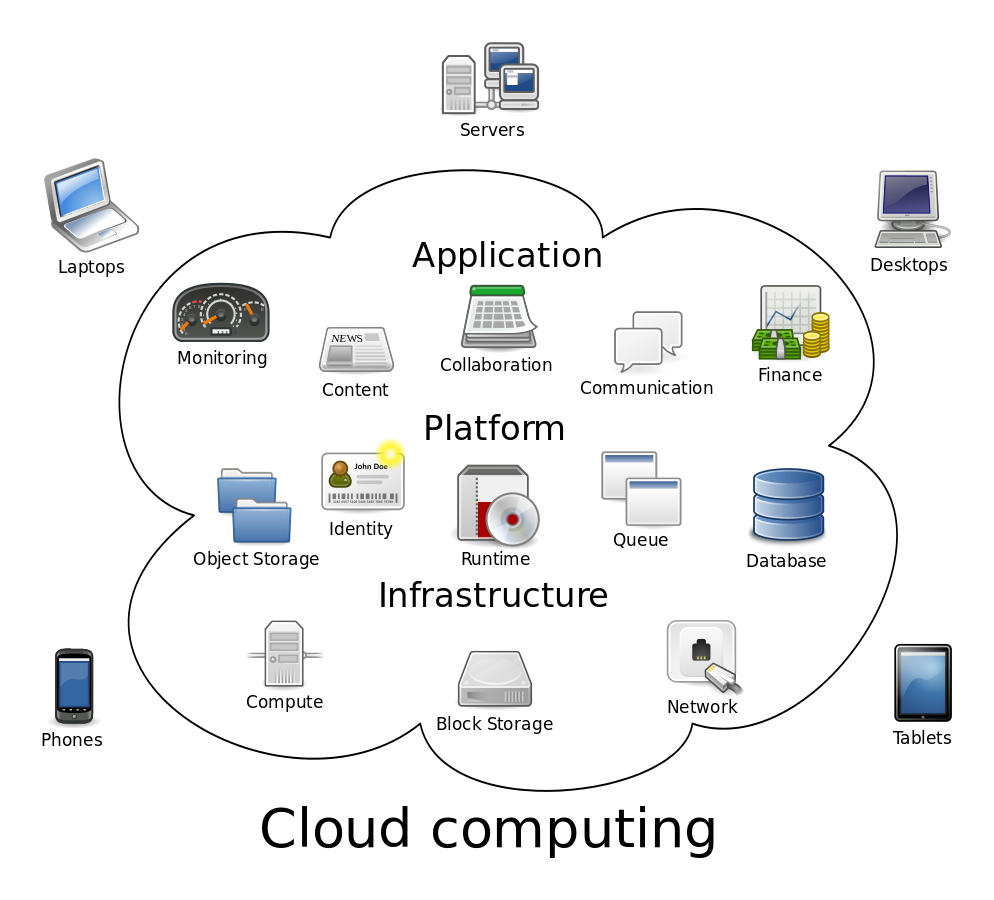
\includegraphics[width=10cm]{images/cc.png}
\caption{\label{fig:cc}Cloud Computing.}
\end{figure} 

The services provided via the cloud can be classified into 3 types:
\subsection{Software As A Service(SAAS)}
Software as a service (SaaS) is a software distribution model in which a third-party provider hosts applications and makes them available to customers over the Internet. SaaS removes the need for organizations to install and run applications on their own computers or in their own data centers. This eliminates the expense of hardware acquisition, provisioning and maintenance, as well as software licensing, installation and support. This kind of service provides the maximum level of abstraction where the user only has to provide an input and recieve output from an application provided by a cloud provider.

\subsection{Platform As A Service(PAAS)}
In a PaaS model, a cloud provider delivers hardware and software tools, usually those needed for developing and hosting new applications. This kind of service works at a lower level abstraction than SAAS, here the provider provides the hardware and the software environment required for users to develop and host an application of their own.

\subsection{Infrastructure As A Service(IAAS)}
In an IaaS model, a third-party provider hosts hardware, software, servers, storage and other infrastructure components on behalf of its users. This works at the lowest level of abstraction where the provider only takes care of the hardware maintainance and the users have to create the required evironment and software as per their requirement. IaaS platforms offer highly scalable resources that can be adjusted on-demand. This makes IaaS well-suited for workloads that are temporary, experimental or change unexpected.

\section{Communication Between Cloud And Device}
Considering the increasing number of mobile devices and their dependence on the cloud it is important to make sure the modes of communication are efficient and ensure on time delivery. The methods of communication can be broadly classified into 2 types:
\subsection{Pull Technology}
Pulling is a style of network communication where the initial request for data originates from the client, and then is responded to by the server. Pull requests form the foundation of network computing, where many clients request data from centralised servers. Pull is used extensively on the Internet for HTTP page requests from websites. A push can also be simulated using multiple pulls within a short amount of time. For example, when pulling POP3 email messages from a server, a client can make regular pull requests every few minutes. To the user, the email then appears to be pushed, as emails appear to arrive close to real-time. The tradeoff is this places a heavier load on both the server and network in order to function correctly. 
\subsection{Push Technology}
Push, or server push, describes a style of Internet-based communication where the request for a given transaction is initiated by the publisher or central server. Push services are often based on information preferences expressed in advance. This is called a publish/subscribe model. A client "subscribes" to various information "channels" provided by a server; whenever new content is available on one of those channels, the server pushes that information out to the client.

A push can also be simulated using multiple pulls within a short amount of time. For example, when pulling POP3 email messages from a server, a client can make regular pull requests every few minutes. To the user, the email then appears to be pushed, as emails appear to arrive close to real-time. The tradeoff is this places a heavier load on both the server and network in order to function correctly.

Another way of simulating push using pull is long pollling. This is used particularly under circumstances where a real push is not possible, such as sites with security policies that require rejection of incoming HTTP/S requests. In this method the client sends a request to the server but the server need not reply instantly but may wait till it has relevant data and as soon as the server sends a reply the client sends another request. Long polling gets rid of the laatency seen in the previous method.

\textbf{General Usage: }Push technology is generally used in synchronous conferencing, instant messaging, email, etc. The SMTP mail protocol is a push protocol, the last step of mail where the client gets the mail from the mail server uses a pull protocol like POP3 or IMAP.
\subsubsection{Hosted Push Services} 
Several companies provide push notification handling as a service. Here the application developer dosn't have to deal with details like queing of messages. Few of the major hosted push services are:
\begin{itemize}
    \item Apple Push Notification Service.
    \item Google Cloud Messaging.
    \item Xtremepush.
  \end{itemize}
\section{Cloud To Device Messaging(C2DM)}
C2DM the predecessor of GCM was released in 2010 and was first featured in Android 2.2. Some of the features presented by C2DM were:\\
\textbf{Features:}
      \begin{itemize}
      		\item When messages are received on the Android client, the
system will wake up the application via an Intent broadcast, and pass the message data.
		\item Developers are encouraged to
send short messages, essentially notifying the mobile
application that updated information can be retrieved
from the server.
		\item Maximum number of messages that can be sent is approximately 200,000 per day. This limit could be increased if required but was not encouraged.
	\end{itemize}
\textbf{Disadvantages:} 
      	\begin{itemize}
      		\item Certain features, such as sending messages to
multiple clients, is not supported. Messages could not be addressed to groups or topics.
		\item The development environment and API could be better. Seeing the possibility of improvment, another push notification library called Simple-C2DM was developed at the same time. Simple-C2DM had simpler APIs and was implemented with a higher level of abstraction.
		\item In certain cases.
quite a big increase in response times for some requests was seen.
	\end{itemize}
\section{Google Cloud Messaging(GCM)}
Google Cloud Messaging (GCM) is a free service that enables developers
to send messages between servers and client apps. This includes
downstream messages from servers to client apps, and upstream
messages from client apps to servers. The architecture of GCM includes 3 main components:
\begin{figure}
\centering
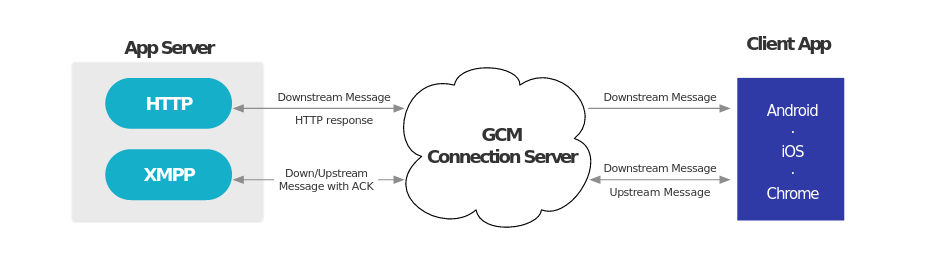
\includegraphics[width=15cm]{images/arch.png}
\caption{\label{fig:arch}GCM Architecture.}
\end{figure} 
\begin{itemize}
	    \item \textbf{GCM Connection Servers: }These are Google servers that transmit the messages from users' application srver to the client application.
	    \item \textbf{Client Application: }This includes all the instances of the GCM enabled application running on different devices.
	    \item \textbf{Application Server: }This is the server handled by the application developer. The messages to the client applications originate from this server and are sent to the connection servers.
  \end{itemize}

Another key concept of GCM is credentials, The IDs and tokens that are used in GCM to ensure that all parties have been authenticated, and that the message is going to the correct place.\\
\textbf{Credentials:}
\begin{itemize}
	    \item \textbf{Sender ID}: The sender ID is used in the registration process to identify an app server that is permitted to send messages to the client app.
	    \item \textbf{API Key}: An API key saved on the app server that gives the app server authorized access to Google services. In HTTP, the API key is included in the header of POST requests that send messages. In XMPP, the API key is used in the SASL PLAIN authentication request as a password to authenticate the connection.
	    \item \textbf{Application ID}: The client app that is registering to receive messages.
	    \item \textbf{Registration Token}: An ID issued by the GCM connection servers to the client app that allows it to receive messages.
	\end{itemize}
\subsection{GCM Lifecycle}
\begin{figure}[h]
\centering
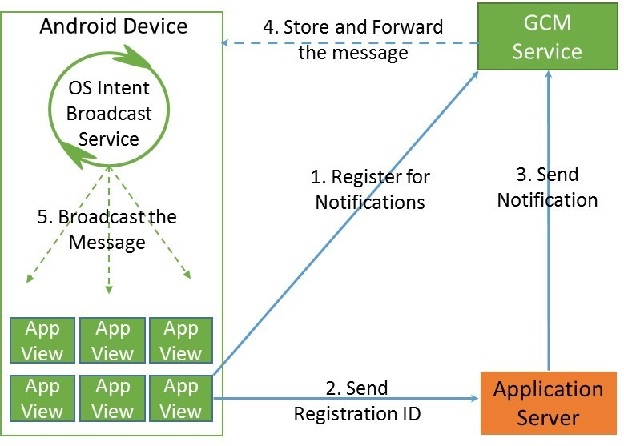
\includegraphics[width=10cm]{images/Steps.jpg}
\caption{\label{fig:arch}GCM Lifecycle.}
\end{figure} 
\subsubsection{Lifecycle Steps: }
\begin{itemize}
	\item Registering Client Application
	\item Send and Recieve downstream messages
		\begin{itemize}
			\item The app server sends a message to GCM connection servers.
			\item The GCM connection server enqueues and stores the message if the device is offline.
			\item When the device is online, the GCM connection server sends the message to the device.
			\item On the device, the client app receives the message according to the platform-specific implementation.
		\end{itemize}
	\item Send and receive upstream messages. This is available only if you use XMPP connection servers
		\begin{itemize}
			\item On the device, the client app sends messages to the XMPP connection server.
			\item The XMPP connection server enqueues and stores the message if the server is disconnected.
			\item When the app server is re-connected, the XMPP connection server sends the message to the app server.
		\end{itemize}
\end{itemize}
\subsection{Registering Client Aplications}
To verify that they can send and receive messages, client apps must register with GCM. In this process, the client obtains a unique registration token and passes it to the app server, which stores the token and sends an acknowledgement back to the client app. The registration token exchanged in this process is the same client app instance identifier that the app server uses to send messages to the particular client.
\begin{itemize}
	\item The client app obtains a registration token using the Instance ID API. The call to this API must have the authorized entity set to your app server's sender ID, and the scope set to the appropriate value for GCM 
	\item The client app passes the registration token to the app server.
	\item The app server saves the registration token and acknowledges to the client app that the process completed successfully
\end{itemize}
In case the server is unable to do its part of the handshaking, the application must retry sending the token or delete it.
\subsubsection{Retry Using Exponential Backoff}
 In case the registration fails, the client app must use exponential backoff to retry i.e. the app must wait double the time it waited on the last try every time.  The retries exponentially increase the waiting time up to a certain threshold. The idea is that if the server is down temporarily, it is not overwhelmed with requests hitting at the same time when it comes back up.
 \newpage
 \begin{figure}[h]
\centering
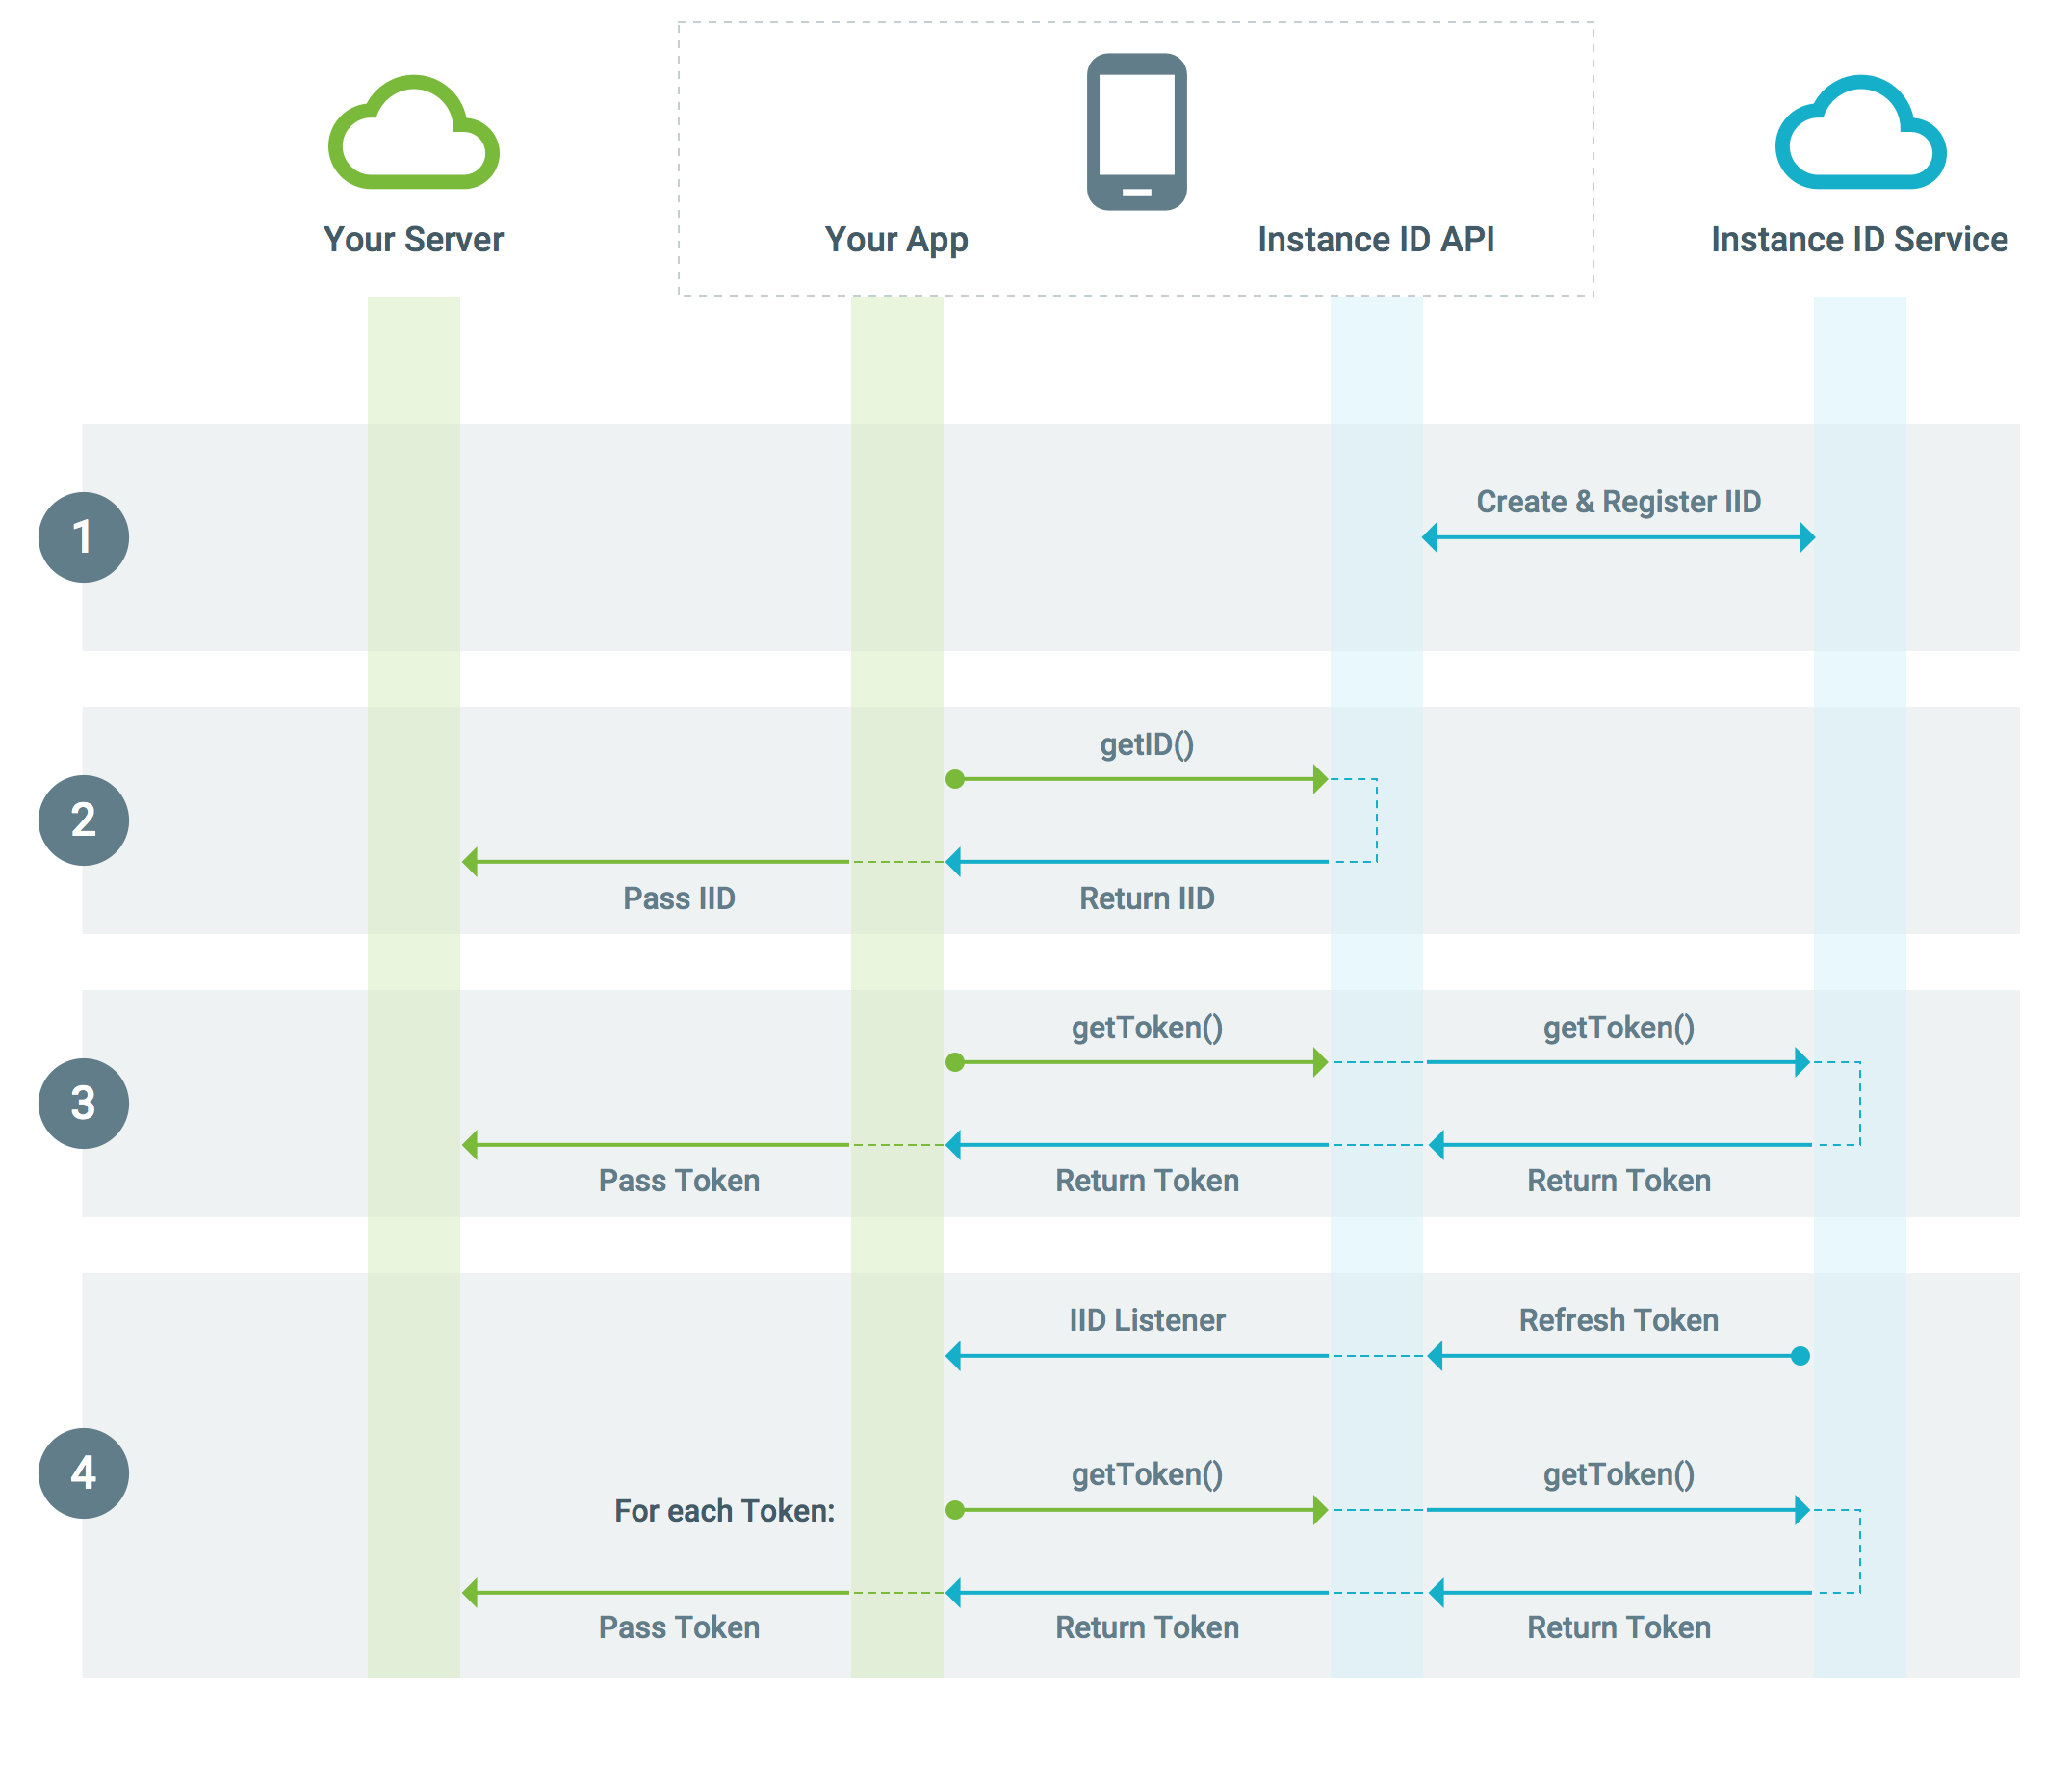
\includegraphics[width=10cm]{images/iid-lifecycle.png}
\caption{\label{fig:iid}Instance ID lifecycle.}
\end{figure}
 \subsubsection{Instance ID API(Android Impletation)} 
 \textbf{Get Instance ID}
\begin{lstlisting}[language=java]
String iid = InstanceID.getInstance(context).getId();
\end{lstlisting}
\textbf{Generate a Token}
\begin{lstlisting}[language=java]
String authorizedEntity = PROJECT_ID; // Project id from Google 
					   //	Developer Console
String scope = "GCM"; // e.g. communicating using GCM, but you 
			 //	can use any
                      // URL-safe characters up to a maximum 
                      //of 1000, or
                      // you can also leave it blank.
String token = InstanceID.getInstance(context).getToken(authorizedEntity,scope);
\end{lstlisting}
\textbf{Refresh Tokens}\\
The Instance ID service periodically refeshes the tokens. It may also do so for the following reasons:
\begin{itemize}
\item security issues.
\item Device information is no longer valid.
\item The Instance ID service is otherwise affected.
\end{itemize}
The app must implement a listener in order to handle these callbacks to refresh tokens.
\begin{lstlisting}[language=java]
public class MyInstanceIDService extends InstanceIDListenerService {
  public void onTokenRefresh() {
    refreshAllTokens();
  }

  private void refreshAllTokens() {
    // assuming you have defined TokenList as
    // some generalized store for your tokens
    ArrayList<TokenList> tokenList = TokensList.get();
    InstanceID iid = InstanceID.getInstance(this);
    for(tokenItem : tokenList) {
      tokenItem.token =
        iid.getToken(tokenItem.authorizedEntity,tokenItem.scope,tokenItem.options);
      // send this tokenItem.token to your server
    }
  }
};
\end{lstlisting}
\subsubsection{Uninstalled Client App Unregistration}
The process of removing tokens of an uninstalled application instance is automated by GCM, but this does not happen instantly. It involves the following steps:
\begin{itemize}
	\item The app server sends a message to GCM connection server addressed to an uninstalled instance.
	\item The GCM connection server sends the message to the GCM client on the device.
	\item The GCM client on the device receives the message and detects that the client app has been uninstalled.
	\item The GCM client on the device informs the GCM connection server that the client app was uninstalled.
	\item The GCM connection server marks the registration token for deletion.
	\item The app server sends a message to GCM for the same instance.
	\item The GCM returns a NotRegistered error message to the app server.
	\item The app server should delete the registration token.
\end{itemize}
\subsection{GCM Connection Servers}
The server side of GCM consists of two components:
\begin{itemize}
	\item Connection Servers 
	\item Application Servers
\end{itemize}
\subsubsection{Application Servers}
Before you can write client apps that use GCM, you must have an application server that meets the following criteria:
\begin{itemize}
	\item Able to communicate with your client.
	\item Able to send properly formatted requests to the GCM connection server.
	\item Able to handle requests and resend them using exponential back-off.
	\item Able to securely store the API key and client registration tokens. Note: never include the API key in any client code.
	\item For XMPP, the server must be able to generate message IDs to uniquely identify each message it sends (GCM HTTP connection server generates message IDs and returns them in the response). XMPP message IDs should be unique per sender ID.
\end{itemize}
\subsubsection{Connection Servers}
Google provides two types of connection servers for GCM, for HTTP and XMPP protocols. The major difference between the two is that XMPP allows both downstream and upstream messages while HTTP allows only downstream messages.\\
\textbf{HTTP Server}\\
To send a message, the application server issues a POST request. A message request is made of 2 parts: HTTP header and HTTP body. The header must contain authorization and content-type. Example:\\
\begin{lstlisting}
Content-Type:application/json
Authorization:key=AIzaSyZ-1u...0GBYzPu7Udno5aA

{
  "to" : "bk3RNwTe3H0:CI2k_HHwgIpoDKCIZvvDMExUdFQ3P1...",
  "data" : {
    ...
  },
}
\end{lstlisting}
\small\textbf{Request Format}\\
The possible types of messages are:
\begin{itemize}
	\item \small\textbf{Send To Sync: } This is the smallest possible message
		\begin{lstlisting}
	{ "to" : "bk3RNwTe3H0:CI2k_HHwgIpoDKCIZvvDMExUdFQ3P1..." }
		\end{lstlisting}
	\item \small\textbf{Message with payload — notification message: }
	\begin{lstlisting}
	{ "notification": {
    				"title": "Portugal vs. Denmark",
    				"text": "5 to 1"
  				},
  	"to" : "bk3RNwTe3H0:CI2k_HHwgIpoDKCIZvvDMExUdFQ3P1..."
	}
		\end{lstlisting} 
	\item \small\textbf{Message with payload — Data message: }
	\begin{lstlisting}
	{ "data": {
    			"score": "5x1",
    			"time": "15:10"
  			},
  	"to" : "bk3RNwTe3H0:CI2k_HHwgIpoDKCIZvvDMExUdFQ3P1..."
	}
		\end{lstlisting} 
\end{itemize}
\textbf{XMPP Server}\\
The Google Cloud Messaging (GCM) Cloud Connection Server (CCS) is an XMPP endpoint that provides a persistent, asynchronous, bidirectional connection to Google servers. The connection can be used to send and receive messages between your server and your users' GCM-connected devices.
The connection has two important requirements:
\begin{itemize}
\item You must initiate a Transport Layer Security (TLS) connection. Note that CCS doesn't currently support the STARTTLS extension.
\item CCS requires a SASL PLAIN authentication mechanism using GCM sender ID and the API key as the password, where the sender ID and API key are the values you gathered when configuring your client app. See the client documentation for your platform for information on obtaining these credentials.
\end{itemize}
The possible types of messages are:
\begin{itemize}
	\item \small\textbf{Send To Sync: } This is the smallest possible message
		\begin{lstlisting}
	<message id="">
  	<gcm xmlns="google:mobile:data">
  	{
      		"to":"REGISTRATION_ID",  
  	}
  	</gcm>
	</message>
		\end{lstlisting}
	\item \small\textbf{Message with payload — notification message: }
	\begin{lstlisting}
	<message id="">
  	<gcm xmlns="google:mobile:data">
  	{
      		"to":"REGISTRATION_ID",  	
     		"notification": {
        		'title': 'Portugal',
        		'text': 'test'
      		},
      		"time_to_live":"600"
	}
  	</gcm>
	</message>
		\end{lstlisting} 
	\item \small\textbf{Message with payload — Data message: }
	\begin{lstlisting}
	<message id="">
  	<gcm xmlns="google:mobile:data">
  	{
     		"to":"REGISTRATION_ID",
      		"message_id":"m-1366082849205"
      		"data":
      		{
        	  "hello":"world",
      		}
      		"time_to_live":"600",
      		"delay_while_idle": true/false,
      		"delivery_receipt_requested": true/false
  	}
  	</gcm>
	</message>
		\end{lstlisting} 
\end{itemize}
\section{Performance Analysis}
In GCM, push notifications to the same device are throttled using token bucket scheme. From the following graphs we can see that the bucket holds 20 tokens and is replenished at a rate of once every 180 seconds. Furthermore, the bucket appears to be completely replenished (randomly) every 0 to 90 minutes. When the bucket is out of tokens, push notifications are dropped instead of queued.
\begin{figure}[h]
\centering
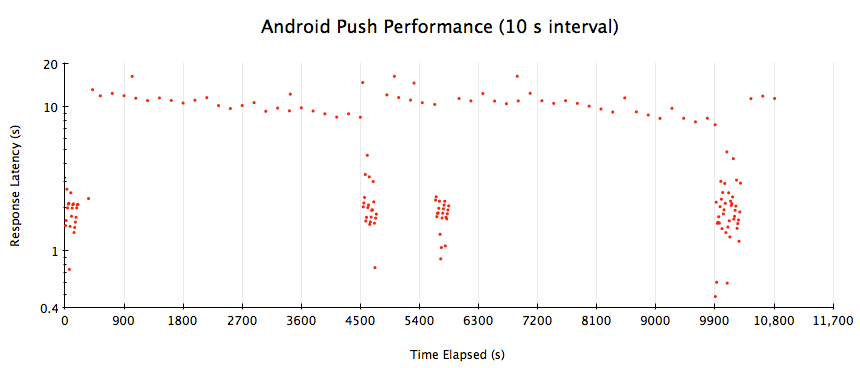
\includegraphics[width=8cm]{images/graph1.png}
\caption{\label{fig:g1}GCM Performance(10s interval).}
\end{figure}
\begin{figure}[h]
\centering
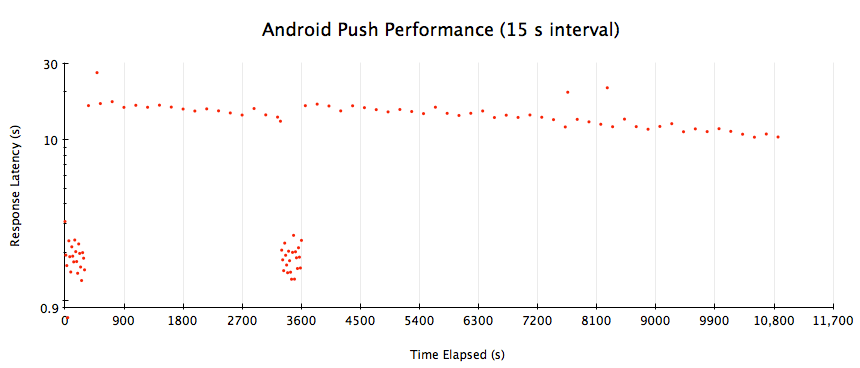
\includegraphics[width=8cm]{images/graph2.png}
\caption{\label{fig:g2}GCM Performance(15s interval).}
\end{figure}
\begin{figure}[h]
\centering
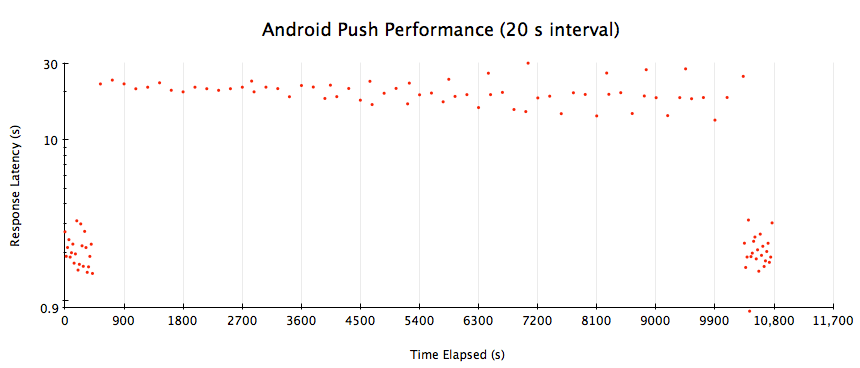
\includegraphics[width=8cm]{images/graph3.png}
\caption{\label{fig:g3}GCM Performance(20s interval).}
\end{figure}
\section{Firebase Cloud Messaging(FCM)}
\begin{figure}[!htb]
\centering
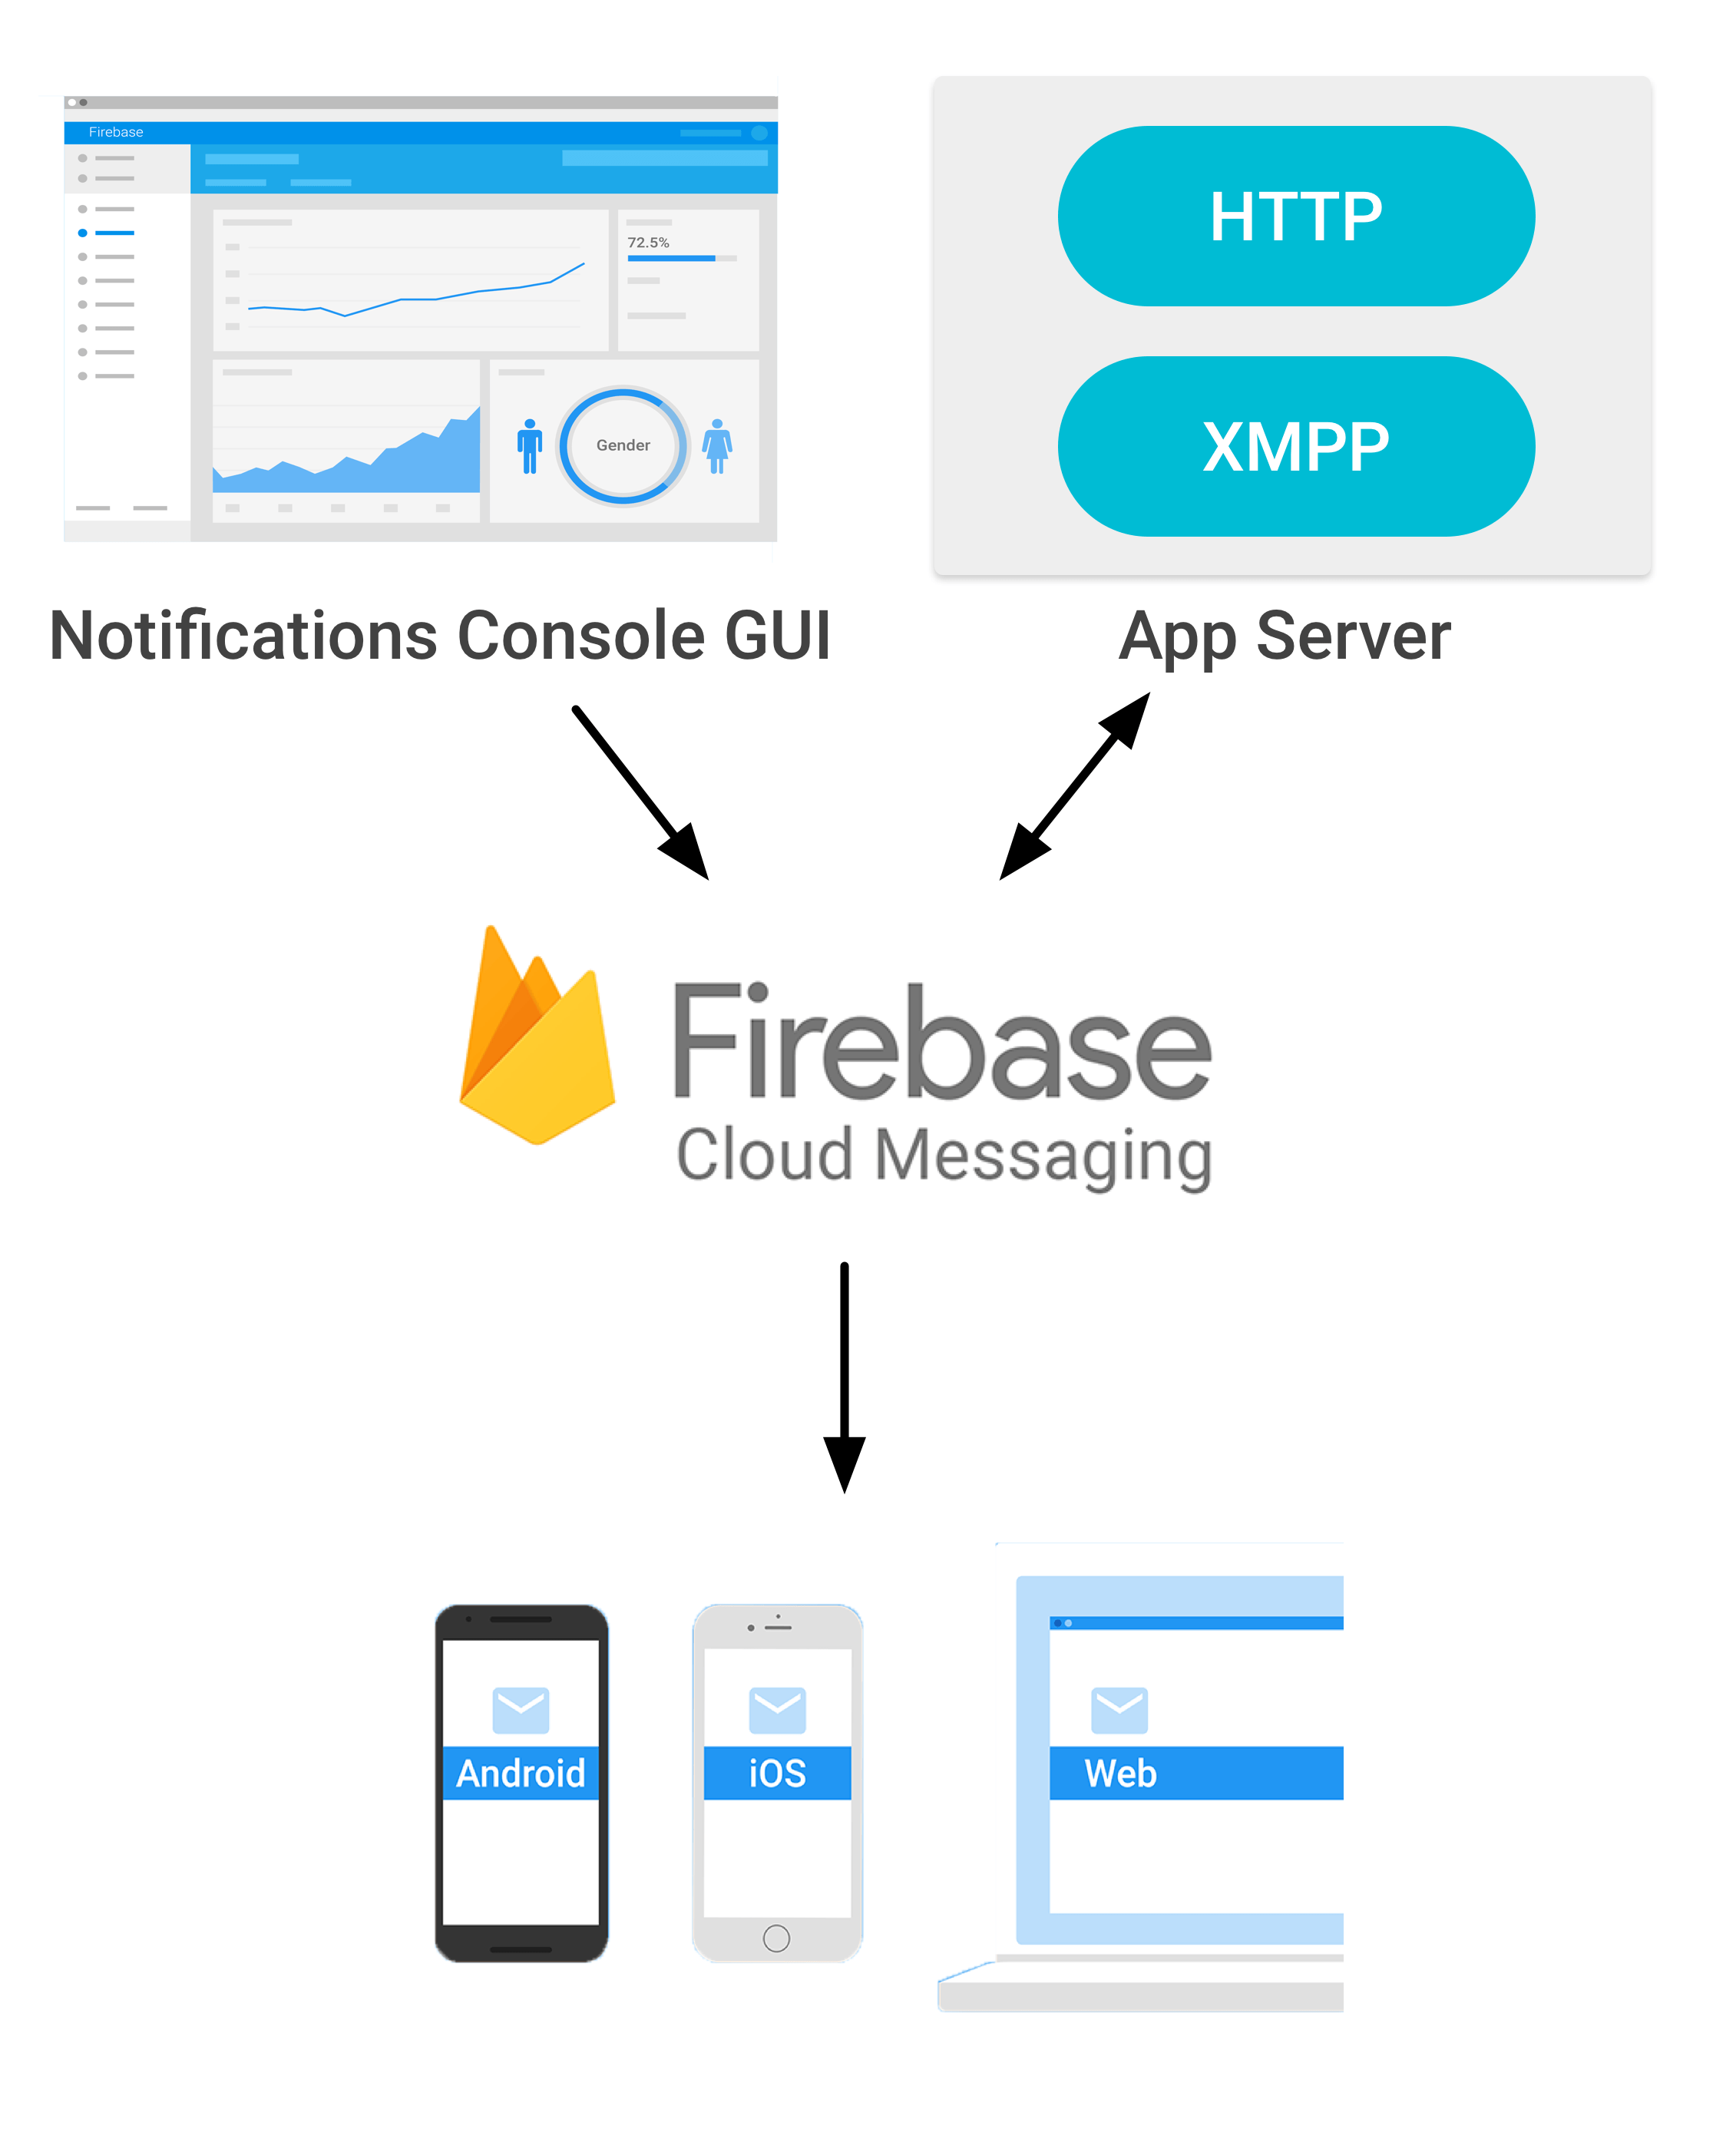
\includegraphics[width=5cm]{images/fcm.png}
\caption{\label{fig:fcm}FCM architecture.}
\end{figure}
Firebase Cloud Platform inherits GCM’s core infrastructure but simplifies the client development. Developers no longer needs to write their own registration or subscription retry logic. FCM includes a web console called Firebase Notifications which allows users to send notifications without an App server.\\
Firebase covers all that mobile developers need to build, maintain and scale a mobile app on all platforms (even on iOS): from Storage and databases to innovative tools like Remote Config and Test Lab.\\
Firebase also presents some performance improvements, it has an average response latency on 250ms and  95\% delivery rate which is a huge improvement when compared to 10s and 40\% on GCM.
\section{Conclusion}
A study on GCM reveals that it is not suitable for time sensitive and/or “must-deliver-to-all” app
scenarios since it does not guarantee a timely message arrival even when a reliable
connection to Google’s GCM servers on the client device exists. GCM is suitable for the application scenarios
where random multicasting is sufficient, such as crowdsourcing
systems. But with the arival of FCM it will be possible to use it for time sensitive and “must-deliver-to-all” app
scenarios.   
\bibliography{../common/seminar}
\bibliographystyle{ieeetr}
\end{document}